


\section{Related Work}

\todo need a table that compares us with related work (!)

\todo Improving operating system kernels to scale

\todo Limitations of the POSIX socket API

\todo User-level networking

\todo Protocol offload engines

\todo Energy-proportionality.   Have a graph that shows the energy-proportionality of a dynamic core approach.


\section{Design Principles}

\begin{figure}
\hspace*{-0.25in}\centering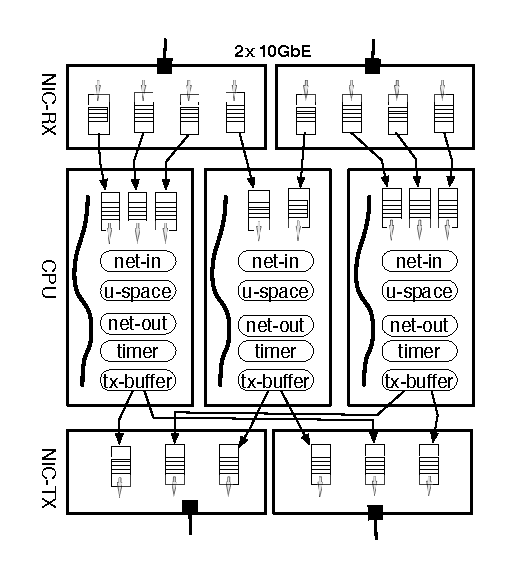
\includegraphics{figs/queues-cores.eps}
\caption{Example of IX scaling across two NICs interfaces, 8 NIC RX queues, and 3 CPU hardware threads.} 
\label{fig:queues-cores}
\end{figure}



\todo Separation of control and data planes

\todo Coherency-free operations  (ala multikernel~\cite{DBLP:conf/sosp/BaumannBDHIPRSS09})

\todo Dynamic spinning cores : re-define pthread abstraction but use it in a different way

\todo Asynchronous channels (like Megapipe)

\todo Abstraction layers: libevent, libpcap


\section{Implementation}

\todo System Archictecture (Dune~\cite{belay2012dune})

\todo Driver layer

\todo TODO (figures, ...)

\section{Evaluation}


\todo Compare apples-to-apples with Megapipe, and mTCP in terms of microbenchmarks.

\todo Baseline comparison of state-of-the art systems include:  Linux (some recent version, with SO\_REUSEPORT); Megapipe (if possible), mTCP (if possible). 

\todo Microbenchmark: short TCP transactions (echo server, as defined in megapipe).   Goal is to beat mTCP (and therefore all others) hands down.

\todo Benchmark: memcached - compare with FB results (?)

\todo Benchmark: lightttpd -- used by Affinity-Accept and mTCP.  

\todo ngnx: an actually used webserver.


\section{Discussion}
\section{Conclusion}




